\documentclass{beamer}
%
% Choose how your presentation looks.
%
% For more themes, color themes and font themes, see:
% http://deic.uab.es/~iblanes/beamer_gallery/index_by_theme.html
%
\mode<presentation>
{
  \usetheme{Goettingen}      % or try Darmstadt, Madrid, Warsaw, ...
  \usecolortheme{beaver} % or try albatross, beaver, crane, ...
  \usefonttheme{default}  % or try serif, structurebold, ...
  \setbeamertemplate{navigation symbols}{}
  \setbeamertemplate{caption}[numbered]
} 

\usepackage[english]{babel}
\usepackage{ulem}
\usepackage{url}
\usepackage{hyperref}
\usepackage[utf8]{inputenc}
\usepackage[T1]{fontenc}

\title[Modeling Cities]{From City Modeling \\ to General Complex Networks\sm}
\author{Gezhi Xiu}
\institute{IRSGIS, Peking University}
\date{\today}

\begin{document}

\begin{frame}
  \titlepage
  \footnote{Presentation for Prof. Yang-Yu Liu's Interview}
\end{frame}

\begin{frame}{Outline}
 \tableofcontents
\end{frame}

\section{About me}
% 自我介绍,以及研究兴趣和背景
\subsection{In person}
\begin{frame}{About me}
	
	\begin{itemize}
	    \item Ph.D. candidate of GIS, Peking University, advised by Prof. Yu Liu
	    \item B.A. of Mathematics and Applied Mathematics, Peking University, advised by Prof. Kai Xu
	\end{itemize}
\textbf{My current research interests:}
\begin{itemize}
    \item Modeling cities through statistical physics
    \item General complex network theories
\end{itemize}
% stability, controllability, and diffusion processes on networks. 
% My coding skills are fine. I am Python user. Familiar with DL framework PyTorch.
\textbf{Personalities:} 

Strongly motivated, curious, optimistic, geeky
\end{frame}

\subsection{My research field}
\begin{frame}{Modeling cities with complex systems}

\textbf{Goals}

\begin{itemize}
  \item Aim to solve, interpret, and control urban complex systems
  \item Study the underlying principles of interdisciplinary networks
\end{itemize}

\textbf{Concerns}

\begin{itemize}
	\item Population dynamics
	\item Economic complexity
	\item Urban structures
	\item Mobility and epidemics
	\item ......
\end{itemize}
\textbf{Why important? Why complex systems?}
\end{frame}

\begin{frame}{The cross-scale complexity}
    The study of cities need systems biology theories because of the common pursuits of stability, controllability, identification of universality, and the emergence of motifs, etc..
    \begin{figure}
        \centering
        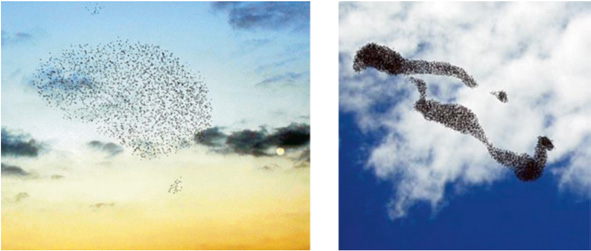
\includegraphics[width = 0.6\linewidth]{Pics/swarm.jpg}
        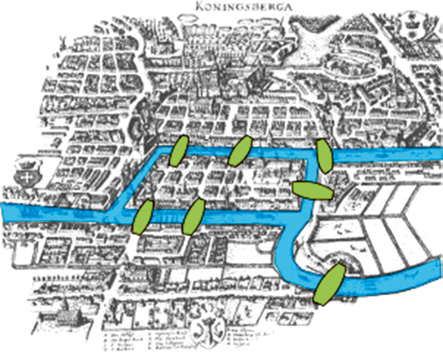
\includegraphics[width = 0.33\linewidth]{Pics/7bridge.jpg}
        \caption{Natural and human complex phenomena. \href{https://link.springer.com/book/10.1007/978-3-319-02024-2}{Source}}
        \label{fig:nathum}
    \end{figure}
\end{frame}

\section{Research works}
% 我的代表性科研工作
\begin{frame}{My research work}

Question: How do cities emerge, grow, and \textit{compete} over space?
\begin{figure}
    \centering
    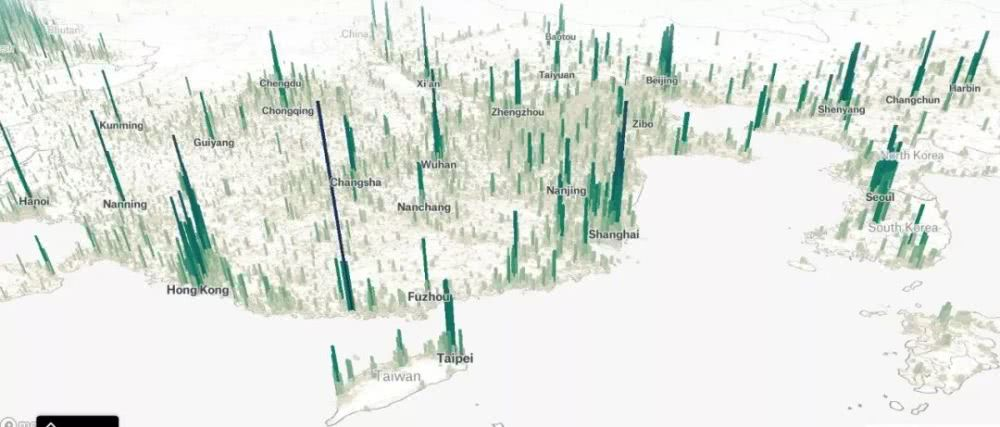
\includegraphics[width = 0.8\textwidth]{Pics/Population_hight_real.jpeg}
    \caption{Population distributions of Eastern China and the Korean Peninsula. \href{https://new.qq.com/rain/a/20190129A06G9C}{\textit{Source link}}}
    \label{fig:pop_real}
\end{figure}
\end{frame}

\subsection{Whys}
\begin{frame}{Why is it important, and what have and haven't been done?}
    % 分成三页ppt。
    Urbanization is complex and diverse, but scaling laws are similar.
    \vspace{0.5cm}
    
    Obvious basic rules behind cities:
    \begin{itemize}
        \item Zipf's law
        \begin{itemize}
            \item The rank size distributions of cities follow a specific form:$P(n) \sim n^{-(1+\gamma)}$, where $\gamma\approx 1$.
        \end{itemize}
        \item Clark's Law
        \begin{itemize}
            \item The spatial distributions of population within a city exponentially decay from urban center: $p(r) \sim P_0e^{-\alpha r}$.
        \end{itemize}
        \item Fractality
        \begin{itemize}
            \item Urban envelopes are fractal.
        \end{itemize}
    \end{itemize}
    
    % Is Zipf's law the same everywhere?
    \begin{center}
        \only<1>{}
        \only<2>{\textbf{How to model? }}
    \end{center}
\end{frame}

\begin{frame}{Why is it important, and what have and haven't been done?}
% 跟上面第一点结合起来
    Existing models have explained the empirical results of Zipf's, Clark's, and scaling laws.
    \begin{itemize}
        \item migration patterns\cite{PhysRevLett.120.108701},
        \item spatial gathering\cite{Li2017Simple}, 
        \item reaction-diffusion\cite{marsili1998interacting}, 
        \\ ......
    \end{itemize}
    Leading to asymptotic behavior of Zipf's law. 
    
    \vspace{0.5cm}
    \begin{center}
        \only<1>{\textbf{Emerge? Grow? Compete?}}
        \only<2>{\textbf{Emerge? Grow? \sout{Compete?}}}
    \end{center}
    
\end{frame}

\begin{frame}{Observations}
Urbanization won't last forever. It is also not driven by pure growth dynamics. It has its own critical dynamics in the percentage of resource. It also has temporal advantages. \textbf{Cities are competitive.}
    \begin{figure}
        \centering
        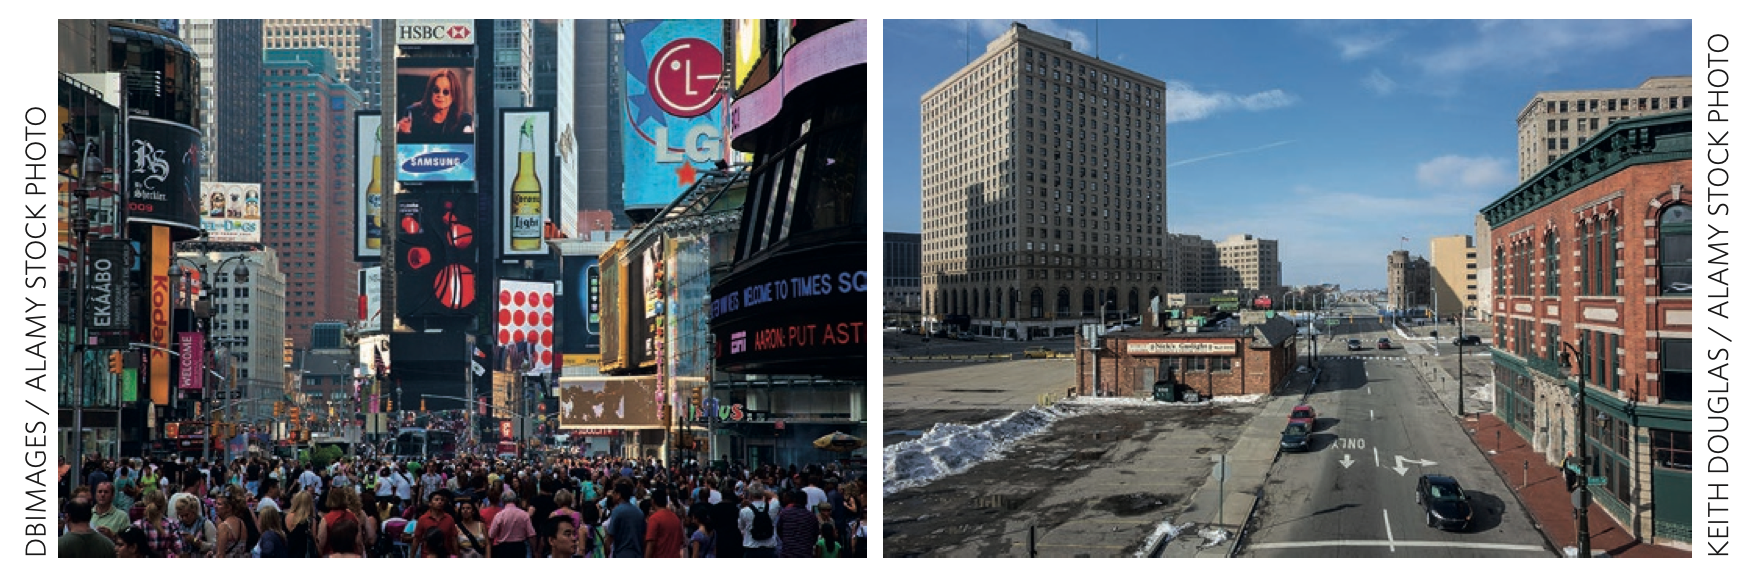
\includegraphics[width = 1\linewidth]{Pics/batty_nyc_detroit.png}
        \caption{NYC \& Detroit. From Michael Batty's thesis, \textit{Diverse cities, successful cities}\cite{batty2017urban}.}
        \label{fig:batty's}
    \end{figure}
    \begin{center}
    \only<1>{Economic complexity and cultural evolution}
    \only<2>{\textbf{We want it simpler.}}
    \end{center}
\end{frame}

\subsection{Formations}
\begin{frame}{Philosophy}
\textbf{Competition for Resource}
    \begin{itemize}
        \item Cities grow because they are \textbf{competitively} better (than rural area or other cities).
        \item The \textbf{total competitiveness} lies in the \textbf{finite active population} $\equiv N^*$.
        % like the IT guys or financial practitioners.
        \item Active people either:
        \begin{itemize}
            \item move in cities and settle somewhere, driven by other actives' attraction, (with rate $\beta_2$);
            \item or establish a new city, (with rate $\beta_1$).
        \end{itemize}
%         \item Active population can be interpreted
% as the people who serve in information industry or finance markets. 
    \end{itemize}
    \begin{center}
        \textbf{Rank relevant intellectuals?}
    \end{center}
\textbf{Competition for Space}
    \begin{itemize}
        \item Once a site is occupied by a city, you can settle here only if you belong here.
    \end{itemize}
\end{frame}

\begin{frame}{Model}
    \begin{figure}
        \centering
        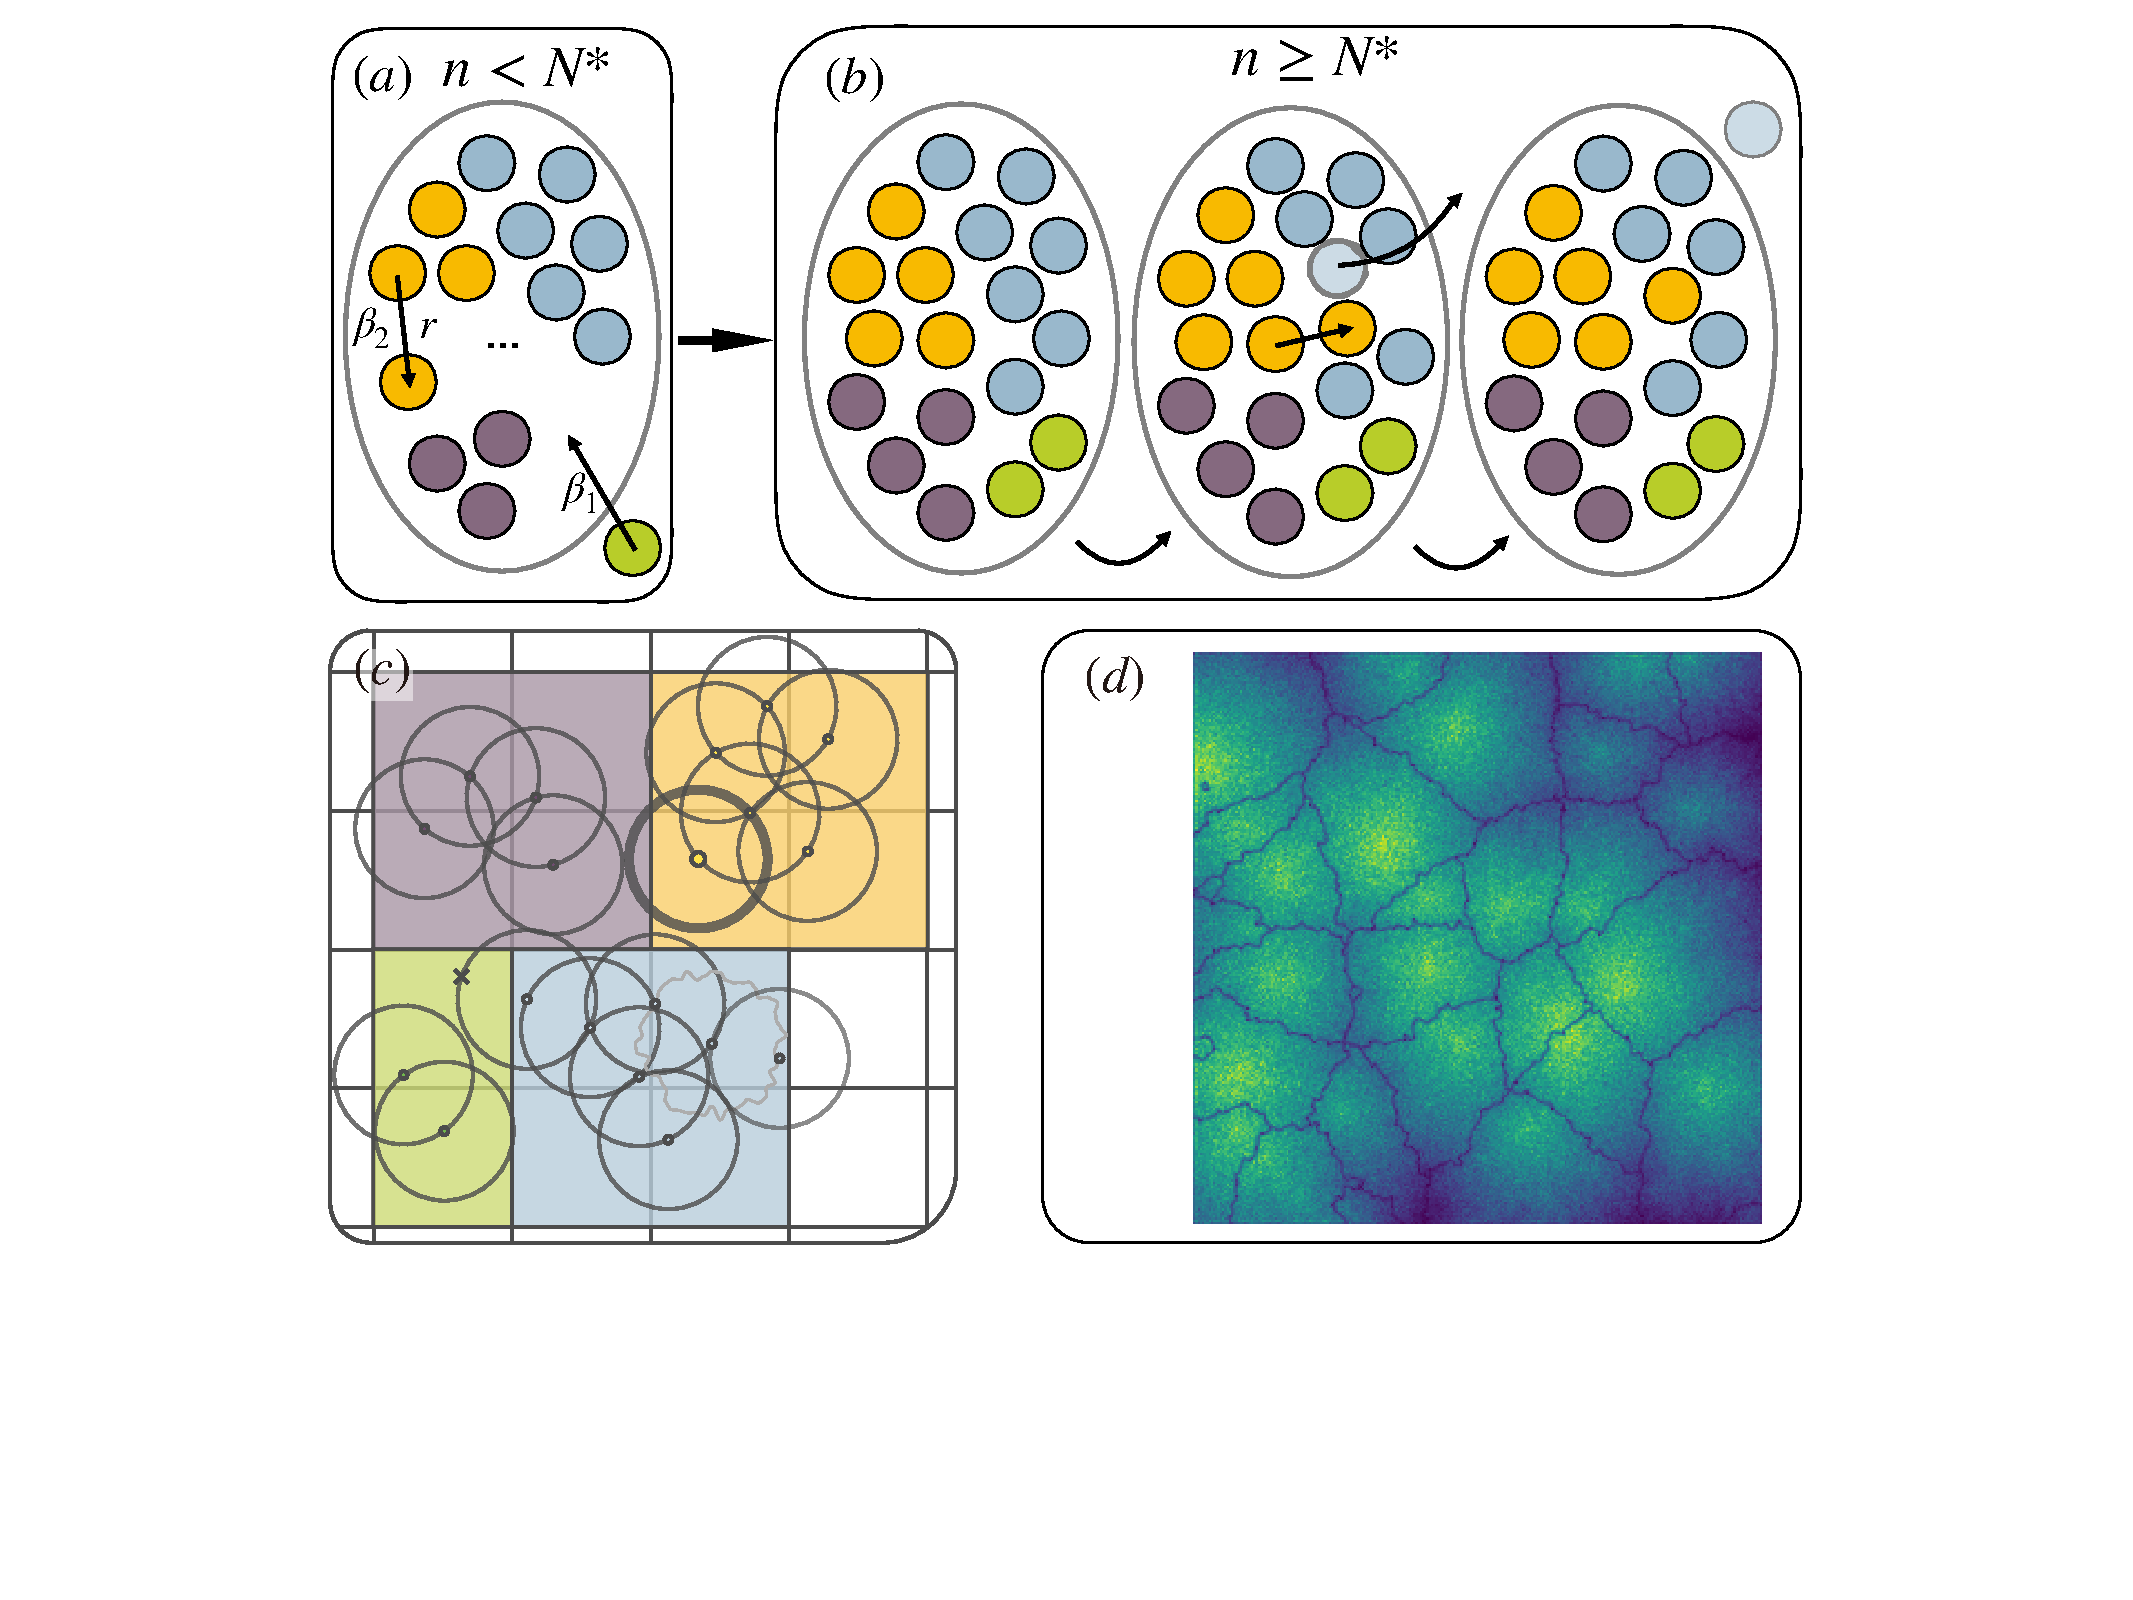
\includegraphics[width = 0.8\linewidth]{Pics/sketchgood.pdf}
        \caption{Model sketch: (a) Speeds of additions of \# of cities and citizens; (b) The role of the memory kernel; (c) Spatial settings; (d) A realization with $\beta_1 = 0.25$, $\beta_2 = 1$, $r=0.5$, $N = 10^5$. }
        \label{fig:sketch}
    \end{figure}
\end{frame}
\begin{frame}{Model}
    \textbf{Notions:}\\
    \hspace{0.25cm}$N_i(t)$: \# of active citizens in $i$'th city at time $t$;\\ \hspace{0.25cm}$k(t)$: \# of cities at time $t$.\\
    \textbf{Rules:}
    \begin{itemize}
        \item The model is based on continuous space and time context.
    \item Growth: restricted preferential attachment. 
    \begin{itemize}
        \item $dN_i(t)/dt = \beta_2 N_i(t) -\delta_{\{\sum N_i = N^*\}} \beta_1k(t)$\\ \hspace{1.8cm}$-\delta_{\{\sum N_i = N^*\}} (N^*-N_i(t))\beta_2$,
        \item $dk(t)/dt = \beta_1k(t)$.
    \end{itemize}
    
    \item Spatial settings:
    \begin{itemize}
        \item Grid blocks. Once a block is taken by one city, citizens from other cities cannot survive.
        \item New city: uniformly, if empty? confirmed.
        \item New active citizen: $(r,\theta)$ from an existing active citizen.
    \end{itemize}
    \item \textit{All parameters:} $r$,$\beta:=\beta_2/\beta_1,$
    \end{itemize}
\end{frame}

\subsection{Results}
\begin{frame}{Results: As an urban system}
    \begin{figure}
    
        \centering
        \begin{minipage}{0.48\linewidth}
        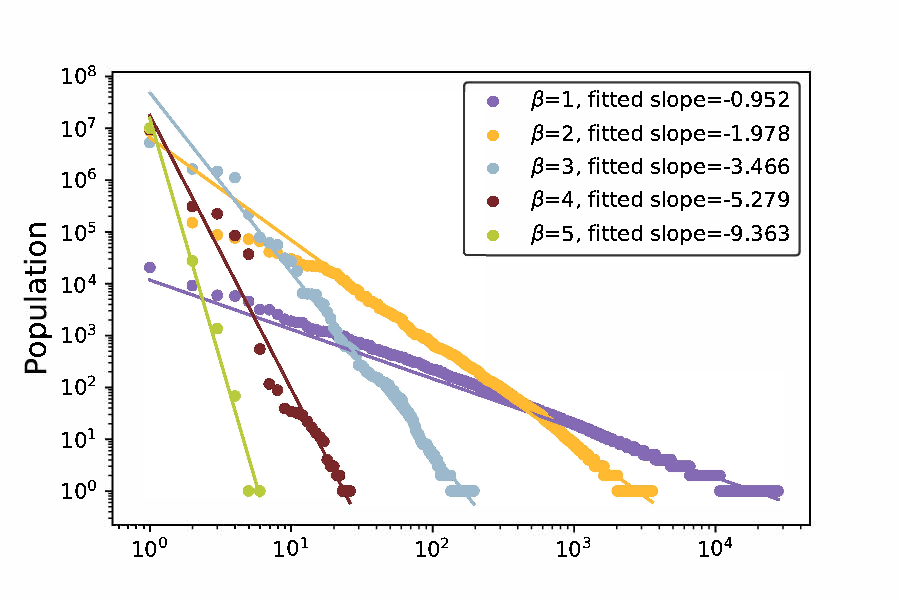
\includegraphics[width = 0.9\linewidth]{Pics/zipf.pdf}
        \caption{Zipf's law of rank size distribution; $\beta:=\beta_2/\beta_1$}
        \end{minipage}
        \begin{minipage}{0.48\linewidth}
        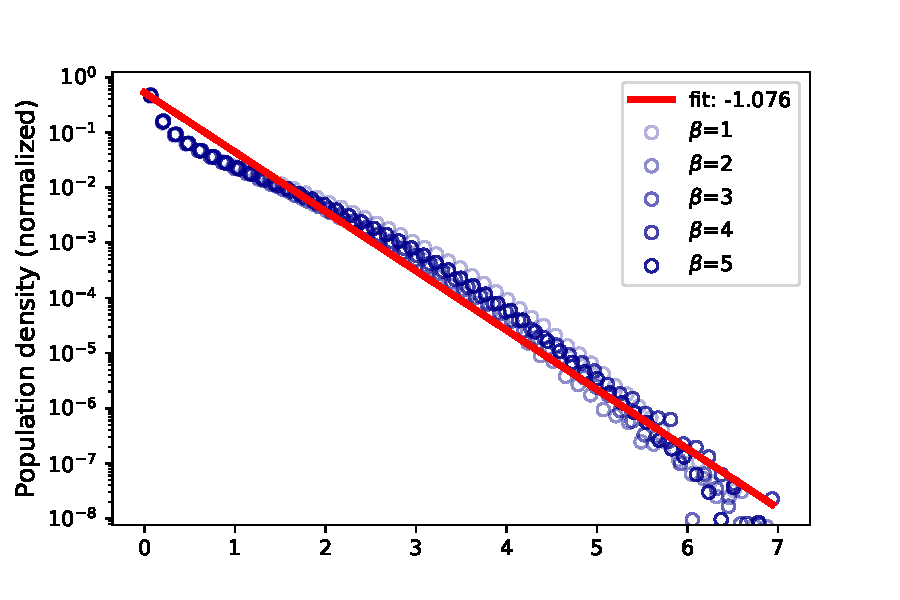
\includegraphics[width = 0.9\linewidth]{Pics/kernal_density.pdf}
        \caption{Clark's law for a city's population density.}
        \label{fig:Zipf}
        \end{minipage}
    \end{figure}
    
    \textbf{SYM is a successful model for urban systems that reformulates Zipf's and Clark's law.}
\end{frame}

\begin{frame}{Results: Competitions for \textbf{resource} and space}
    \textbf{Critical density:}
    \[\rho_{threshold} = k/\beta.\] $\uparrow$ with \# of cities $k$. Survival probability of a site $\downarrow$.
    
When the space is filled, \textbf{Critical population:}
    \[N_{threshold} = 0.5 N^*\]
\textbf{Turnover rate:}
\begin{figure}
    \centering
    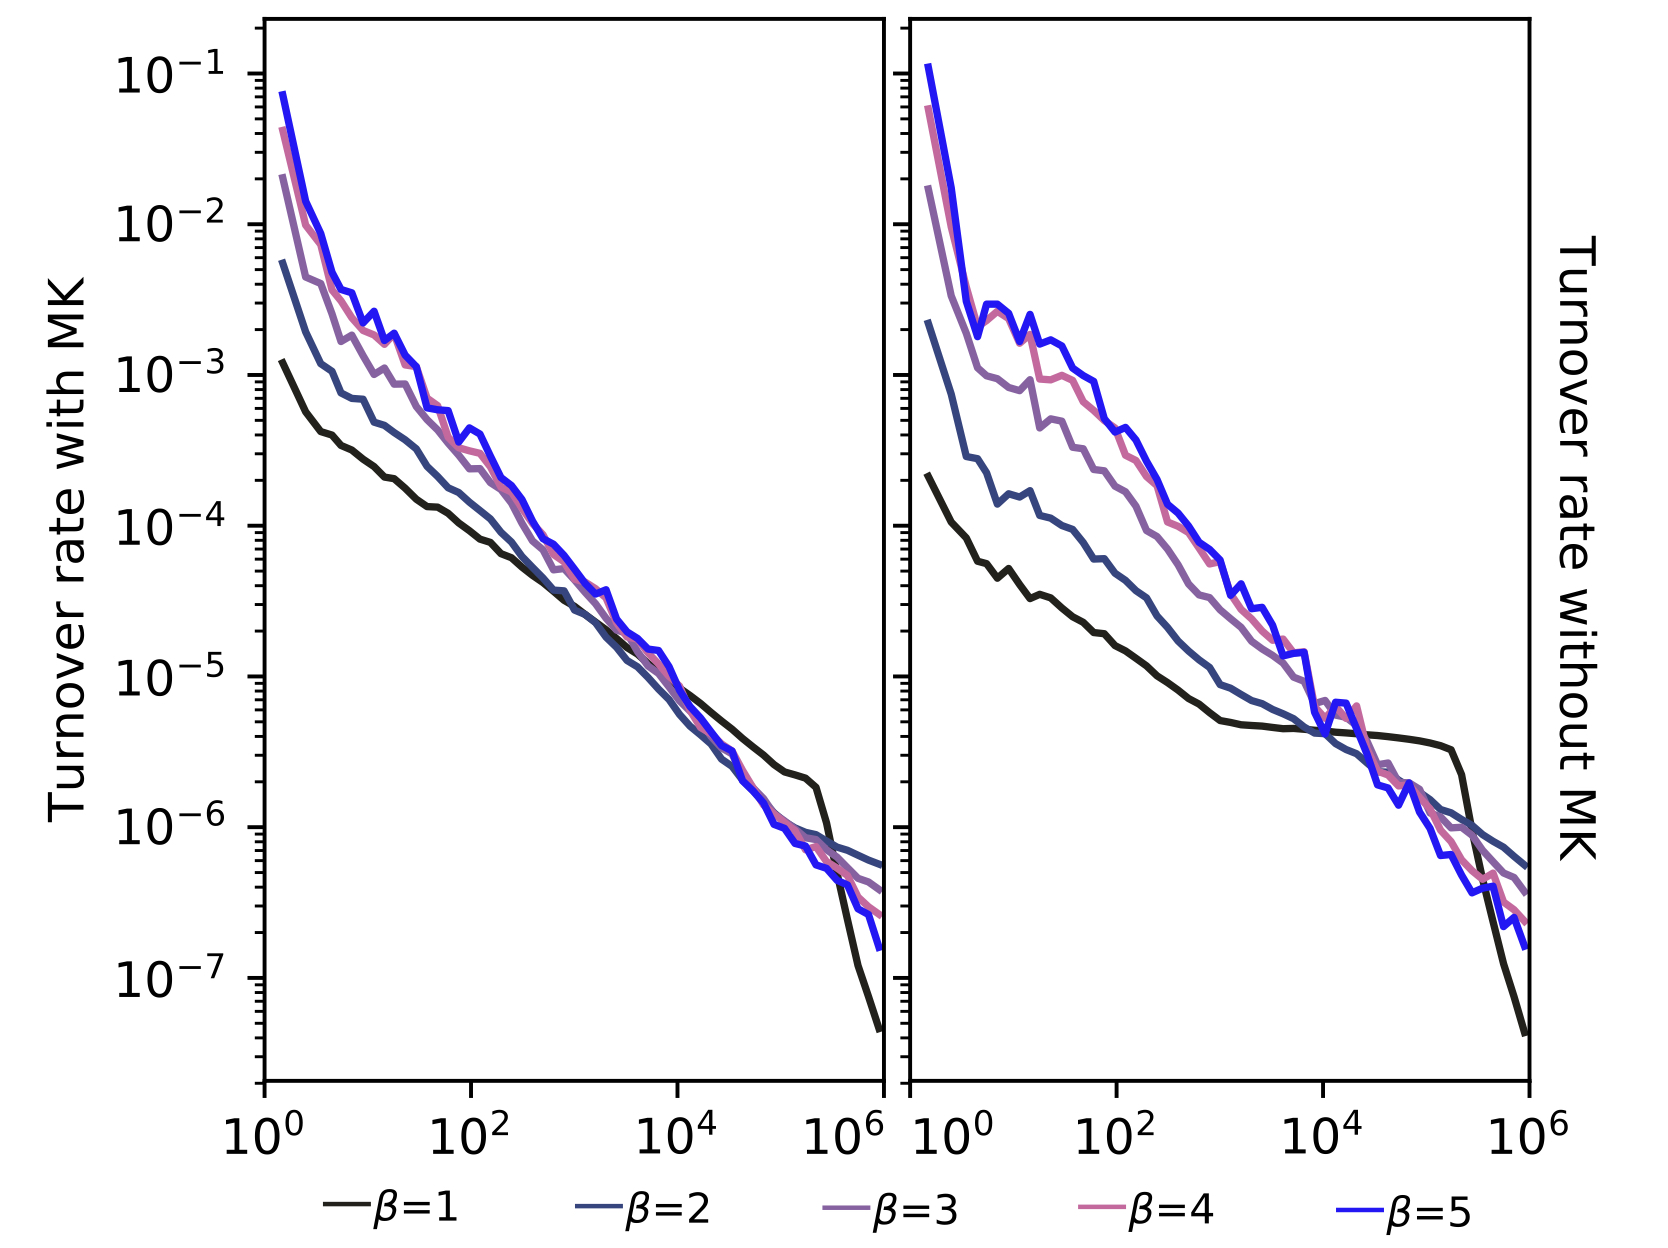
\includegraphics[width = 0.65\linewidth]{Pics/in_one.jpeg}
    \label{fig:turnover}
\end{figure}

\end{frame}

% \begin{frame}{Results: Competitions for resource and \textbf{space}}

% \begin{figure}
%     \centering
%     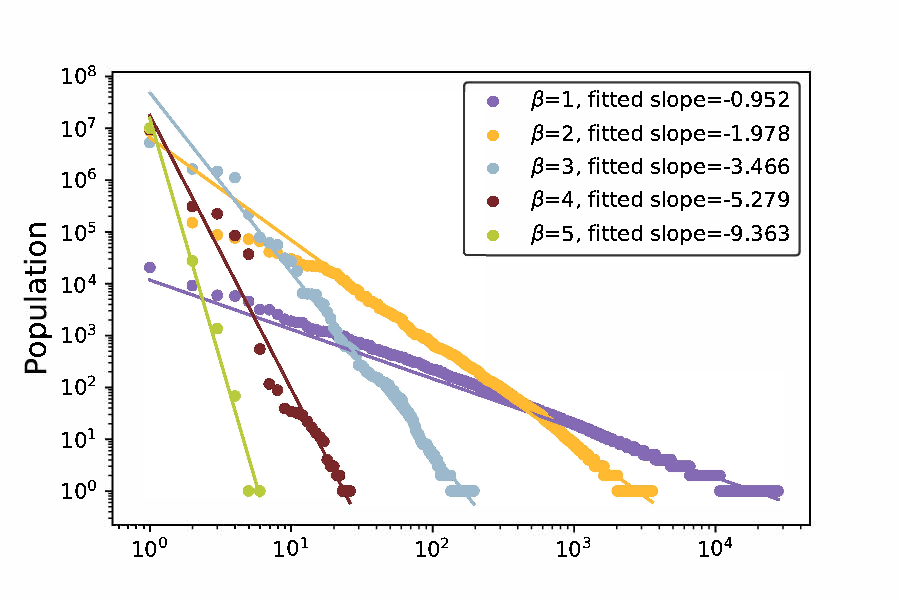
\includegraphics[width = 0.9\linewidth]{Pics/zipf.pdf}
%     \caption{Zipfian exponents are significantly larger when $\beta\uparrow$.}

% \end{figure}
    
% \end{frame}

\begin{frame}{Results: Competitions for resource and \textbf{space}}
\begin{minipage}{0.6\linewidth}
\begin{figure}
    \centering
        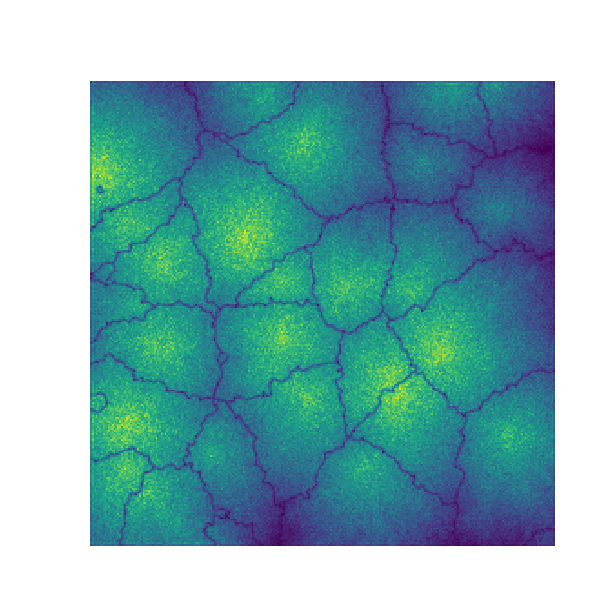
\includegraphics[width = 0.6\linewidth]{Pics/fractal_41_256.pdf}
        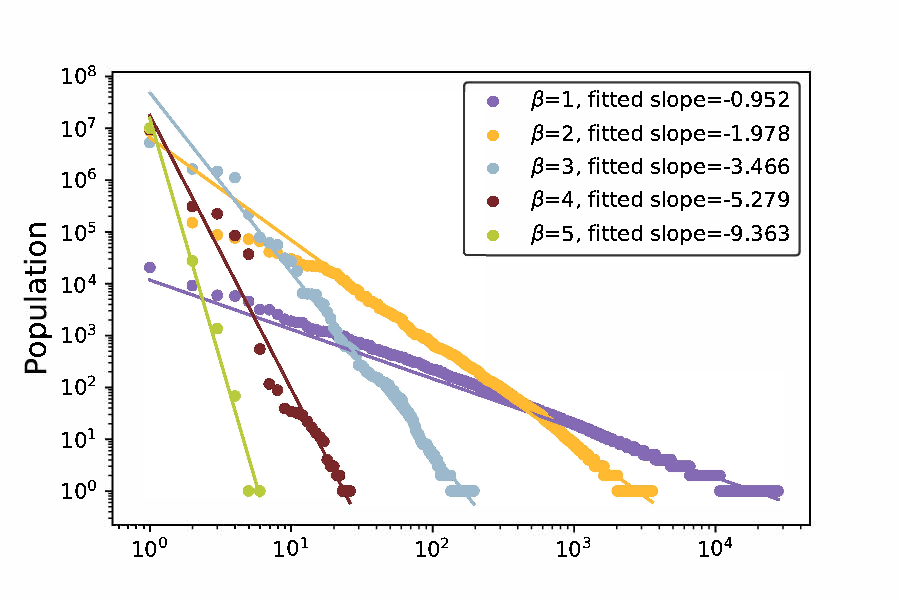
\includegraphics[width = 0.6\linewidth]{Pics/zipf.pdf}
        \caption{\textit{Above:} Fractal edges drawn from SYM. \textit{Below:} The absolute values of the slopes are expected as $\beta$ without a spatial context.}
    
    \label{fig:my_label}
\end{figure}
\end{minipage}
\begin{minipage}{0.38\linewidth}
\begin{itemize}
    \item Small cities are advantageous for spatial competitions.
    \item For large $\beta$'s, the survival probability of small cities decreases rapidly, bring advantages for big cities.
\end{itemize}
\end{minipage}

\end{frame}

\begin{frame}{Our histogram}
    \begin{figure}
        \centering
        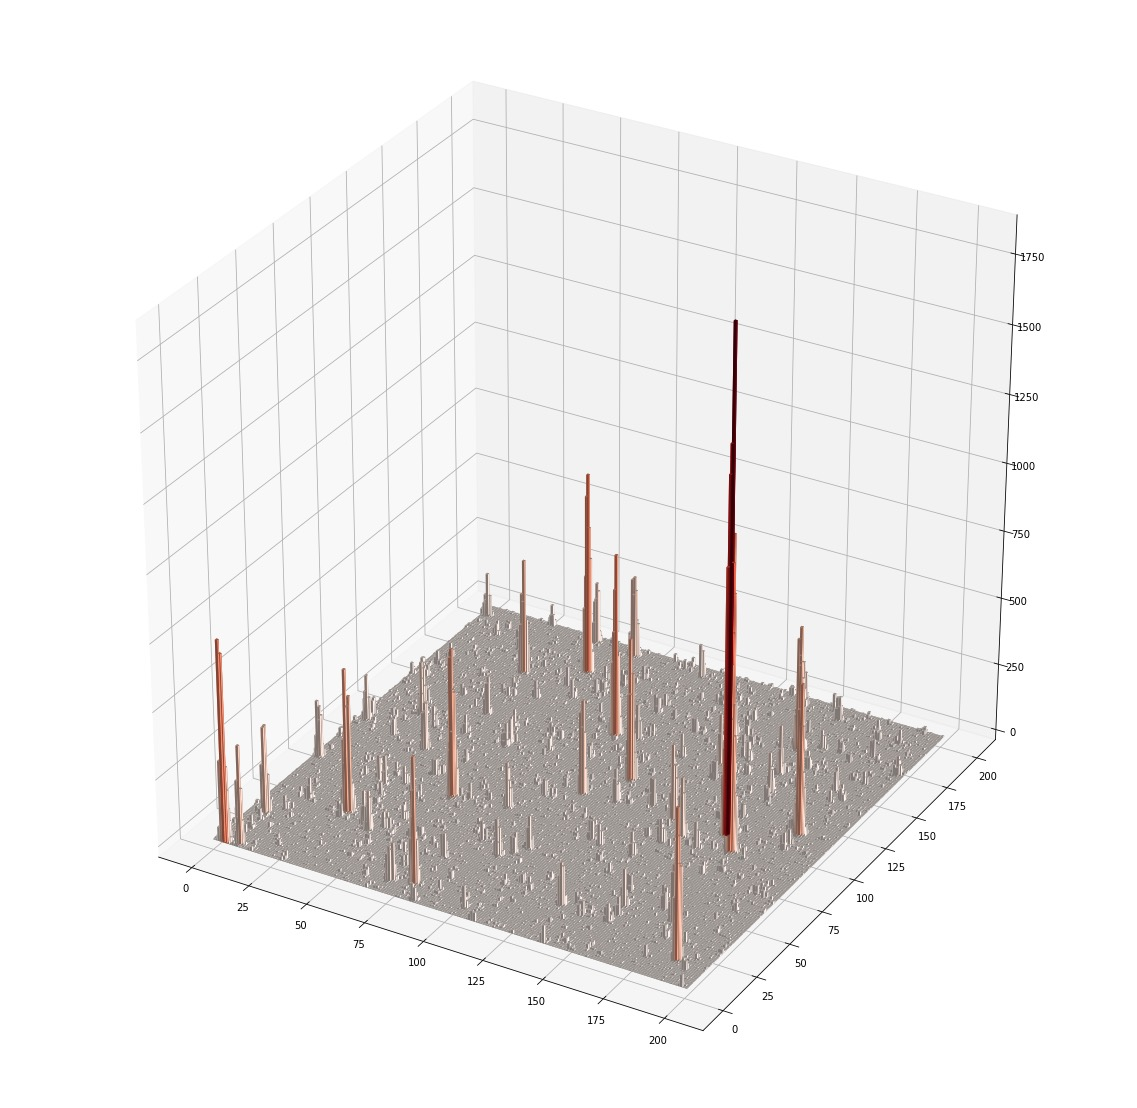
\includegraphics[width = 0.7\linewidth]{Pics/3dhist.jpeg}
        \caption{Simulated result.}
        \label{fig:my3dhist}
    \end{figure}
\end{frame}
\subsection{Insights}
\begin{frame}{Insights}
    \begin{itemize}
        \item The tendency of vicissitudes is strengthened by the restrictions of resource. \item The bottom-up formations of traditional models are not enough to model cities.
        \item Zipf's law with $\gamma \approx 1$?
            \textbf{Not quite!}
        \item Spatial competition has to be taken serious, especially for small areas. 
        \item Critical phenomena from branching process can be broadly adopted.
    \end{itemize}
\end{frame}

\section{Research plans}
% 未来工作计划
\begin{frame}{Research plans: Problems}
    \begin{itemize}
        \item How could complex network theory make it better for urban life?
        \item Dig in complex network, especially structural and temporal heterogeneities of the contact network.
        \item Feeding back: what does space mean for complex networks?
    \end{itemize}
\end{frame}
\subsection{Physics and society}
\begin{frame}{Physics and society}
E.g., how can we interpret and improve \textit{urban traffic networks} through statistical physics?
    \begin{itemize}
        \item The benefits of public transport\cite{buchanan2019benefits}, $T/P = 1-p$
        \item Topology and the spatial evolution of neighborhoods v.s. slums in cities\cite{brelsford2018toward}
        \item Urbanization correlated to hantavirus epidemics
    \end{itemize}
    \begin{figure}
        \centering
        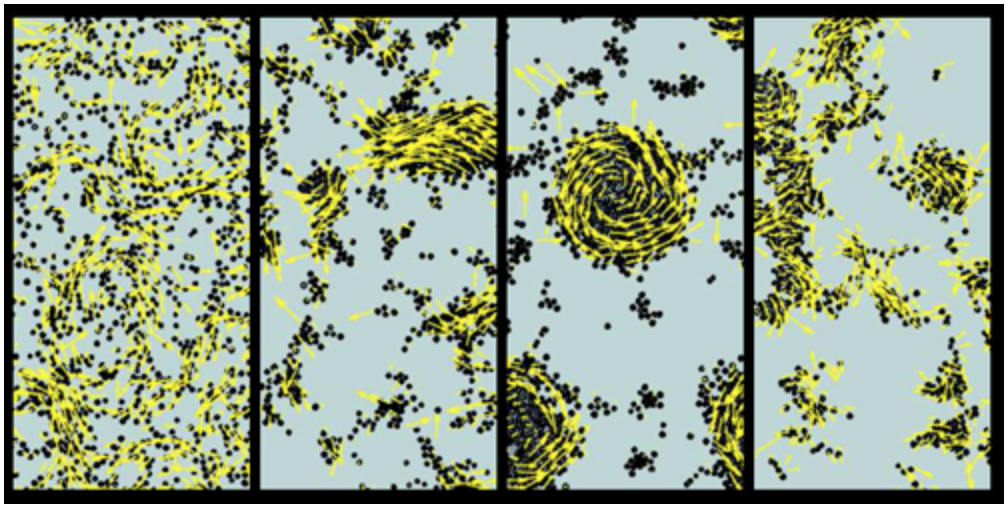
\includegraphics[width = 0.6\linewidth]{Pics/rwprl.png}
        \caption{Collective Dynamics of microbial. H. Karani et al., Phys. Rev. Lett. (2019)}
        \label{fig:rwprl}
    \end{figure}
\end{frame}

\begin{frame}{Physics and society}
    A design for road network generation towards cities without slums: 
    \begin{itemize}
        \item Based on the generation method in \cite{PhysRevLett.100.138702} with different optimization purpose: from \textit{connecting to the network the still unconnected centers using as little as possible road length}, to \textit{a linear combination of connectivity and tendency to get a block surrounded by roads}.
    \end{itemize}
    \begin{figure}
        \centering
        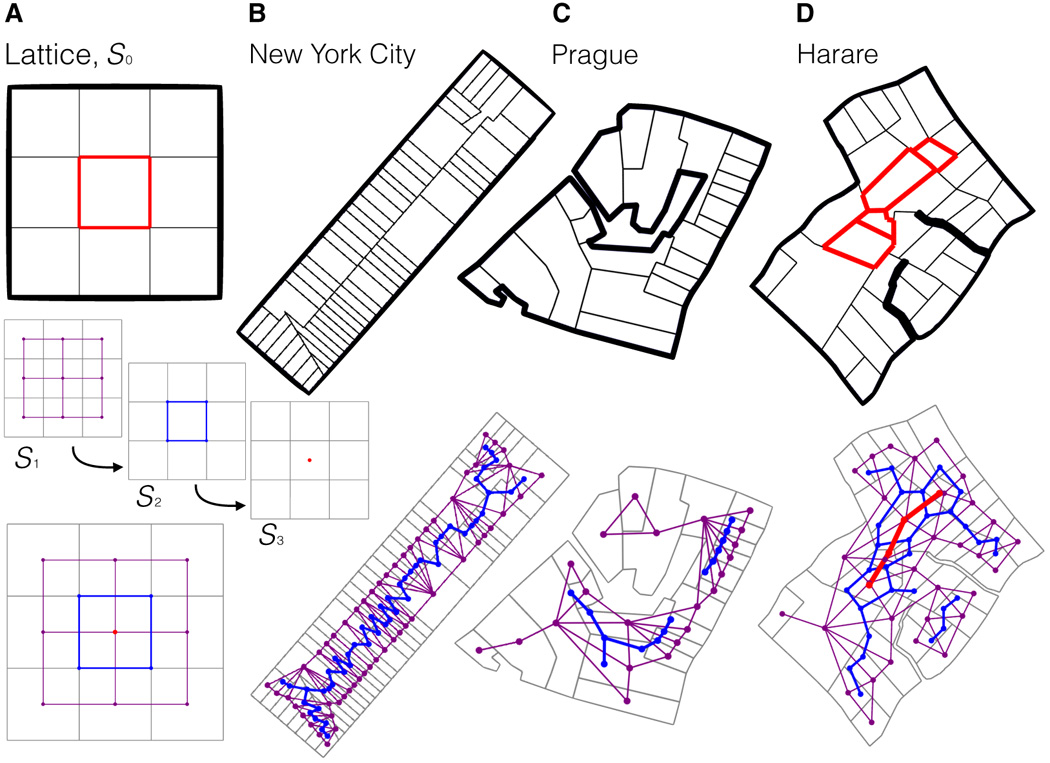
\includegraphics[width = 0.45\linewidth]{Pics/F1.large.jpg}
        \caption{Towards cities without slums, \cite{brelsford2018toward}}
        \label{fig:withoutslum}
    \end{figure}
\end{frame}

\subsection{Structures}
\begin{frame}{Structures in complex systems}
\begin{itemize}
    \item Predictability\cite{sun2020revealing,scarpino2019predictability} through \textit{compression of graphical structures} or \textit{permutation entropy}.
    \item Controllability\cite{liu2011controllability,gao2014target,angulo2019theoretical}
    \item Minimum of complex network\cite{barzel2015constructing}
    \item Geometric renormalization for the growth of modular networks\cite{song2006origins}
    \item ......
    \begin{figure}
        \centering
        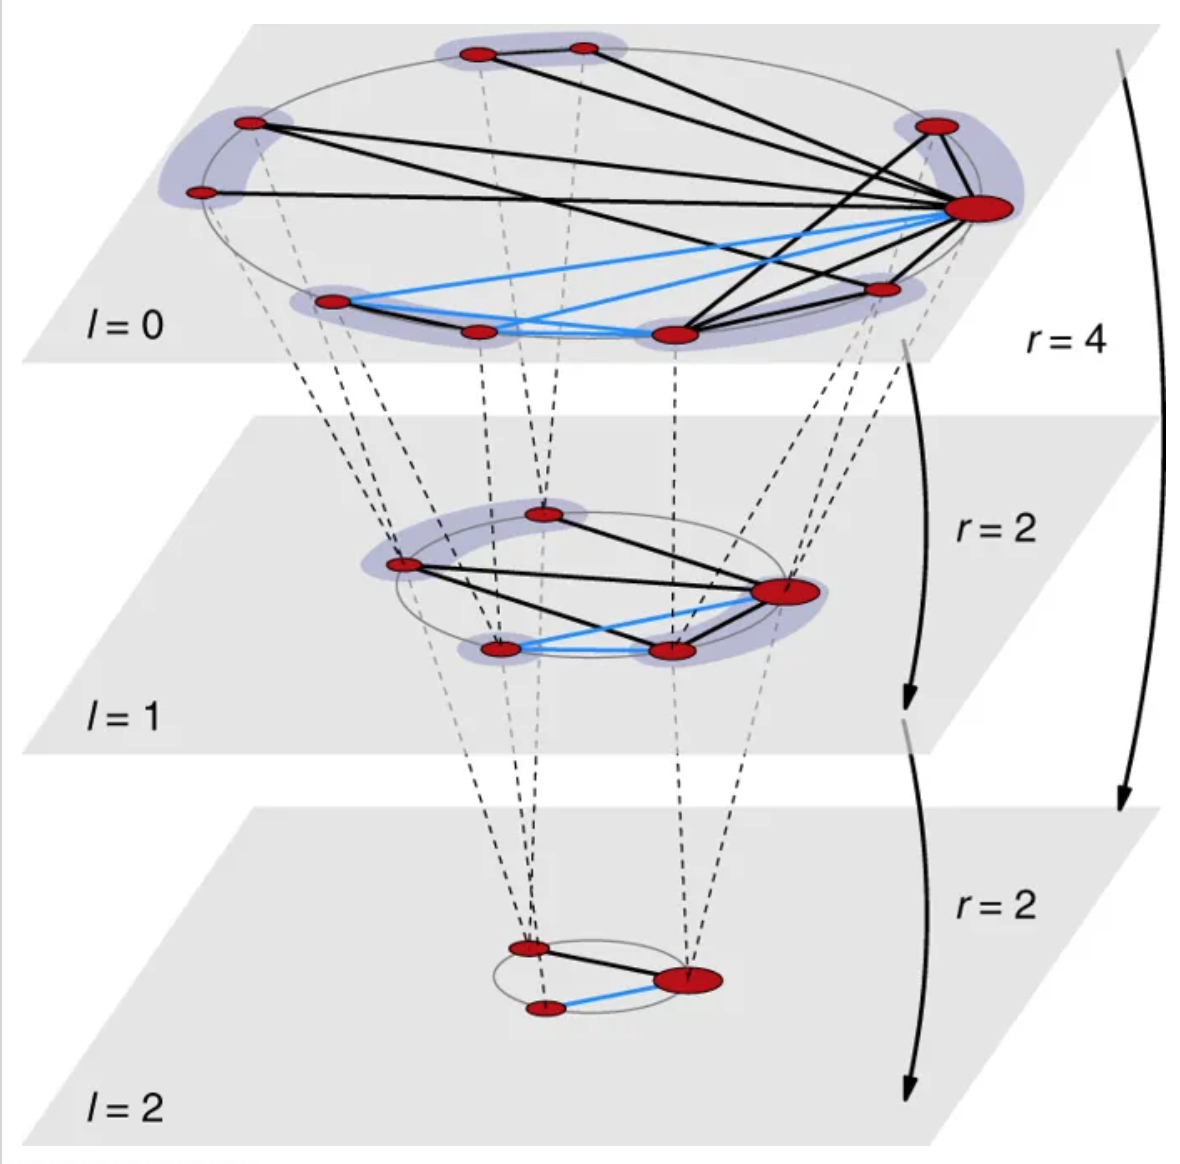
\includegraphics[width = 0.4\linewidth]{Pics/gr.png}
        \caption{Structural transitions of network by renormalizaiton group. From Ref.\cite{garcia2018multiscale}}
        \label{fig:my_label}
    \end{figure}
\end{itemize}
    
\end{frame}

\subsection{Feeding back}

\begin{frame}{Feeding back: What can those beyond links tell network?}

\begin{itemize}
    \item Density-based analysis: carbon emission, spatial structures, anomalous structures(tumors)...
    \item The variations of controllability of network is non-linear...
    \item Spatial networks, represented by epidemic models, are now highly related to human mobility models, as a preface of Physical Review E:
    \begin{figure}
        \centering
        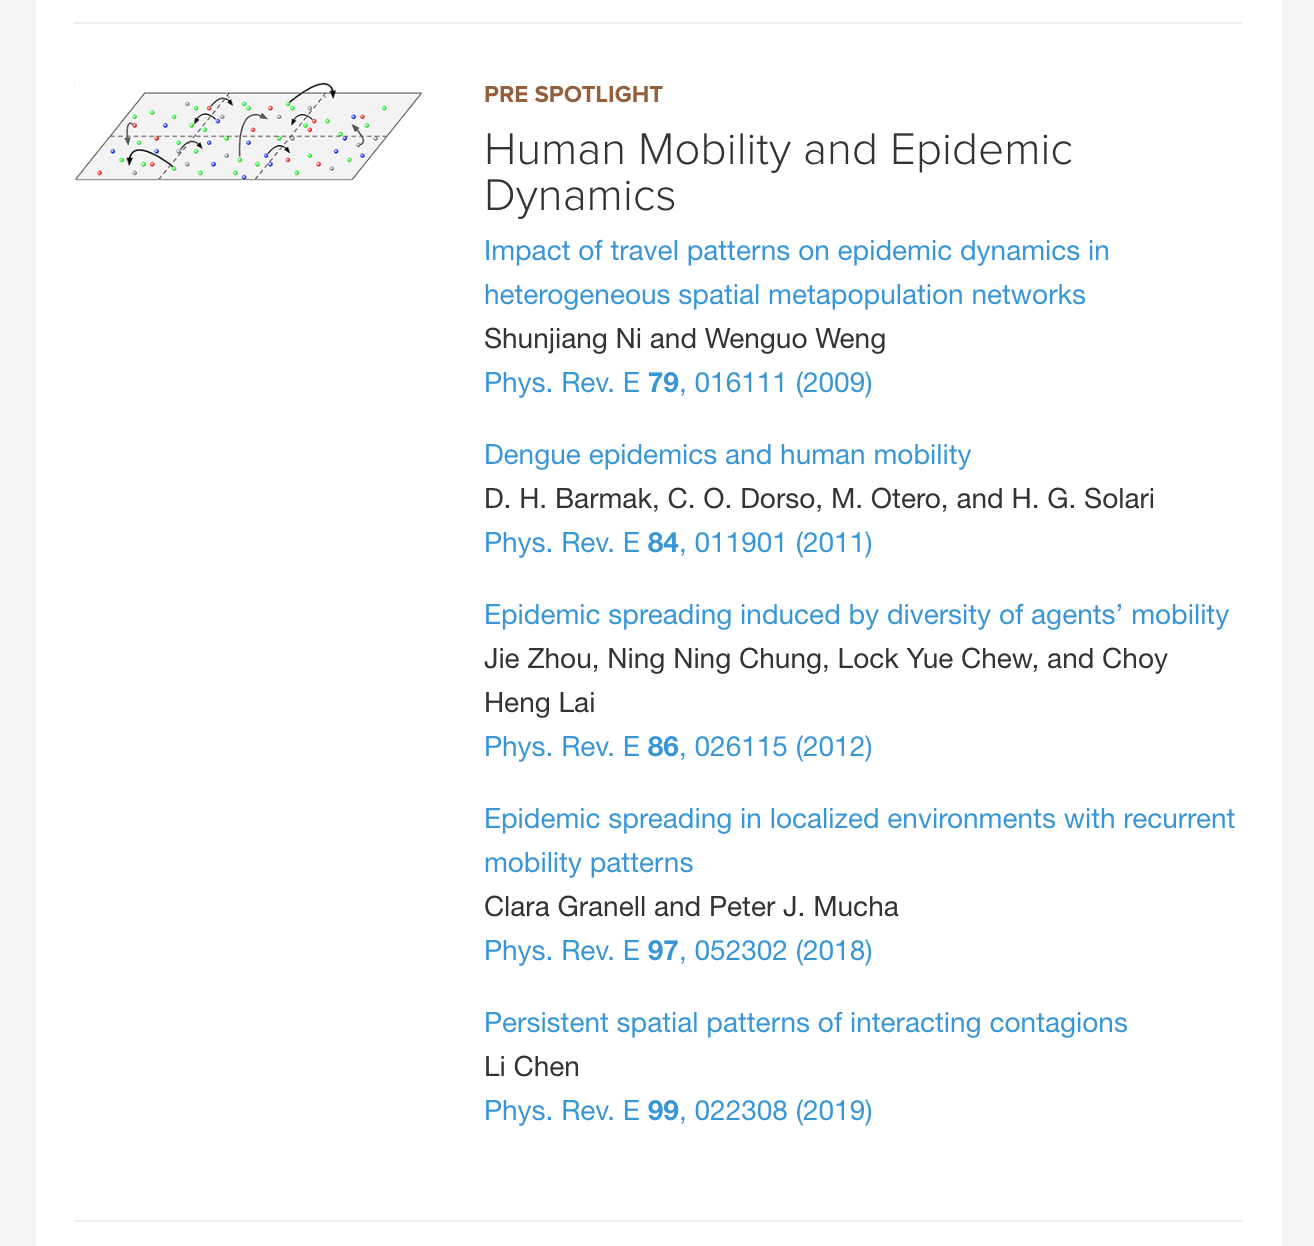
\includegraphics[width = 0.5\linewidth]{Pics/preface.png}
    \end{figure}
\end{itemize}
    
\end{frame}

\begin{frame}{Q1: Density-based versus link-based}
    Various attempts beyond link structures:
    \begin{itemize}
        \item Simplicial models of social contagion
        \begin{itemize}
            \item speed of contagion helps to identify the most vulnerable or dangerous individuals in an outbreak
        \end{itemize}
        \item Contact-Based Model for Epidemic Spreading on Temporal Networks\cite{PhysRevX.9.031017}
        \item My model of SYM
    \end{itemize}
    \begin{figure}
        \centering
        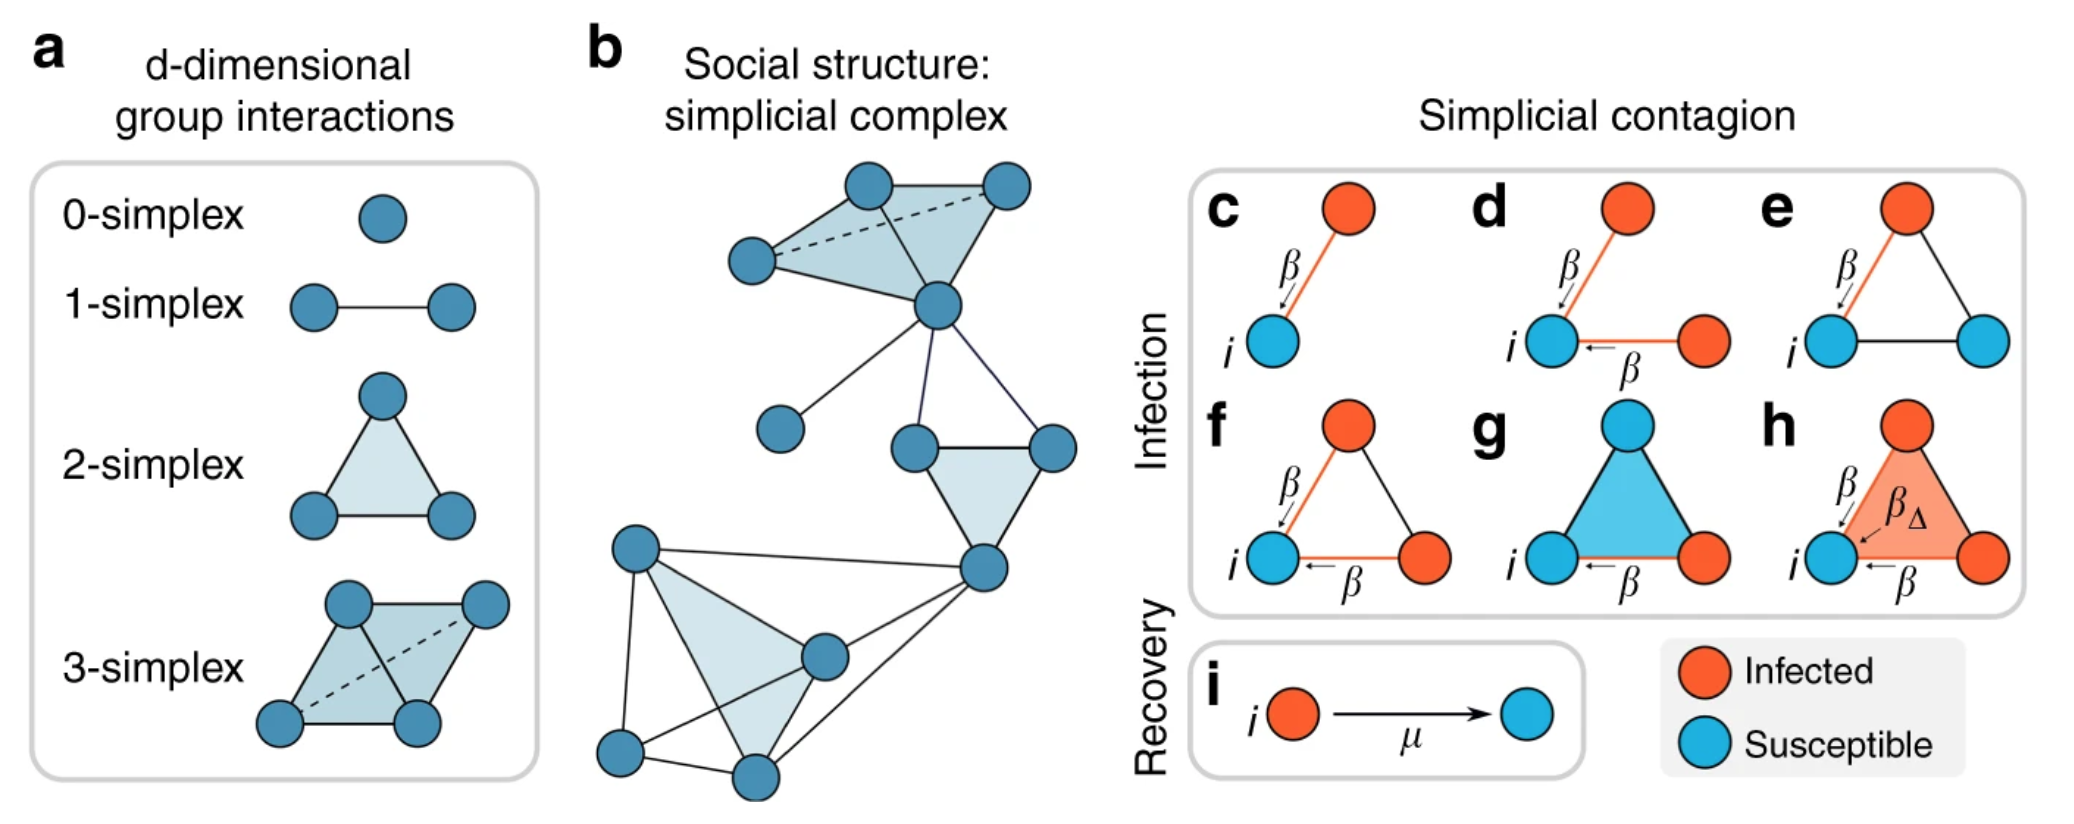
\includegraphics[width = 0.9\linewidth]{Pics/simplicial.png}
        \caption{Simplicial contagion model. \href{https://www.nature.com/articles/s41467-019-10431-6}{Source}}
        \label{fig:my_label}
    \end{figure}
\end{frame}

\begin{frame}{Q2: Function versus threats}
    \begin{figure}
        \begin{minipage}{0.48\linewidth}
            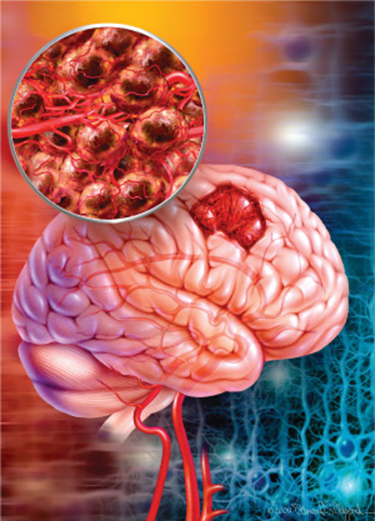
\includegraphics[width = 0.4\linewidth]{Pics/braintumor.jpg}
        \end{minipage}
        \begin{minipage}{0.48\linewidth}
            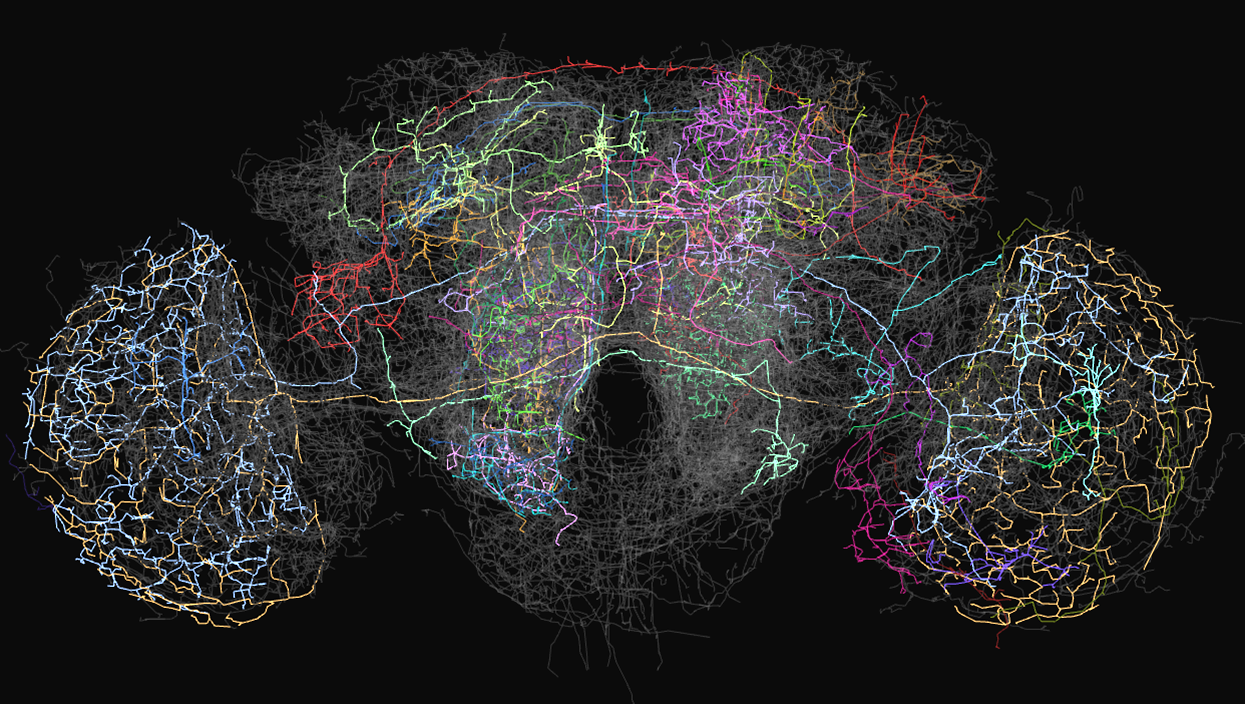
\includegraphics[width = 1\linewidth]{Pics/simple-words-about-the-complex-what-are-neural-networks-1.png}
        \end{minipage}
        \caption{Brain tumor (\href{http://medicalxtourism.com/wp-content/uploads/2014/06/Brain-Cancer-Symptoms-and-Tumor-Survival-Rate-in-UK.jpg}{\textit{source}}), and Neural network(\href{http://gadget.fsetyt.com/wp-content/uploads/2017/06/simple-words-about-the-complex-what-are-neural-networks-1.png}{\textit{source}}). It is interesting how functional organs, e.g., the brain, interconnects more topologically through links, such as synapsis or pipes; while the threat parts, such as tumors in brains and slums in cities, are usually spatial clusters.
        } 
    \end{figure}
    
\end{frame}


\begin{frame}{Q3: What's more?}
    \begin{center}
        \textbf{Let's find out together.}
    \end{center}
\end{frame}

\begin{frame}{Research plans: Timelines}
    \textbf{Timelines:} My visit will start from June or July. 
    \begin{center}
        \begin{tabular}	{|c|c|}
        \hline
        - to 2020-08 & Settle down, material reading,\\ & pick two/three projects \\ \hline
        2020-09 to 2020-10 & Basic experiments, discussions on \\ & values, feasibility, research proposals \\ \hline
        2020-11 to 2021-06 & Finish a work, revalue the aims below\\ \hline
        2021-07 to - & Collaborate on challenging topics\\ \hline 
        \end{tabular}
    \end{center}
    \textbf{Aims:} 
    \begin{itemize}
        \item (Hopefully) Find universal laws that exist both in human societies and microbial;
        \item Improve the theoretical basis of complex network theory;
        \item Give optimizations and solutions to cities with statistical physics.
    \end{itemize} 
\end{frame}


% 感谢
\begin{frame}
\centering
\Large{Thank you for listening!}

\vspace{2cm}
email: xiugz@pku.edu.cn\\
personal page: gxiu.github.io

    
\end{frame}
\bibliographystyle{unsrt}
\bibliography{refs}

\end{document}